\documentclass{article}
\usepackage[utf8]{inputenc}
\usepackage{graphicx}
\usepackage{amsmath}
\title{ECC(Part 1)}
\author{Subha Nawer Pushpita}
\date{January 2021}

\begin{document}

\maketitle

\section{A little Summary}
I will give a little summary of the main thing I loved this week :), I am mainly studying theories and math-heavy things, but also implementing python scripts for RSA and ECC, to have a better grasp of the algorithm, later I wish to implement some ZK based game 
\begin{itemize}
    \item Main theme behind RSA is that multiplication is easy whereas factoring is really hard. So initially this was the reason why it was useful for tasks like encryption or depcryption. Later it turned out the difference of hardness between factoring and multiplication shrinks as we move to larger and larger prime numbers, which made it necessary to come up with something else. If you love number theory, this will be really interesting to dive into :DD
    \item Here comes ECC(Elliptic Curve Cryptography). Most cryptocurrencies including Ethereum and Bitcoin uses this one because a 256-bit elliptic curve private key is just as secure as a 3072-bit RSA private key. Smaller keys are easier to manage and work with. 
    \item An elliptic curve is a curve satisfying the following equation : $y^2=x^3+ax+b$ where $4a^3 + 27b^2 \ne 0$ ( this is to avoid singular points)
    \item The elliptic curve used by Bitcoin, Ethereum, and many other cryptocurrencies is called secp256k1. The equation for the secp256k1 curve is $y^2 = x^3+7$
    \item Some beautiful properties of ECC are point addition and scalar multiplication, I am adding the images of how it works (let’s say we wanna add P and Q)\\
    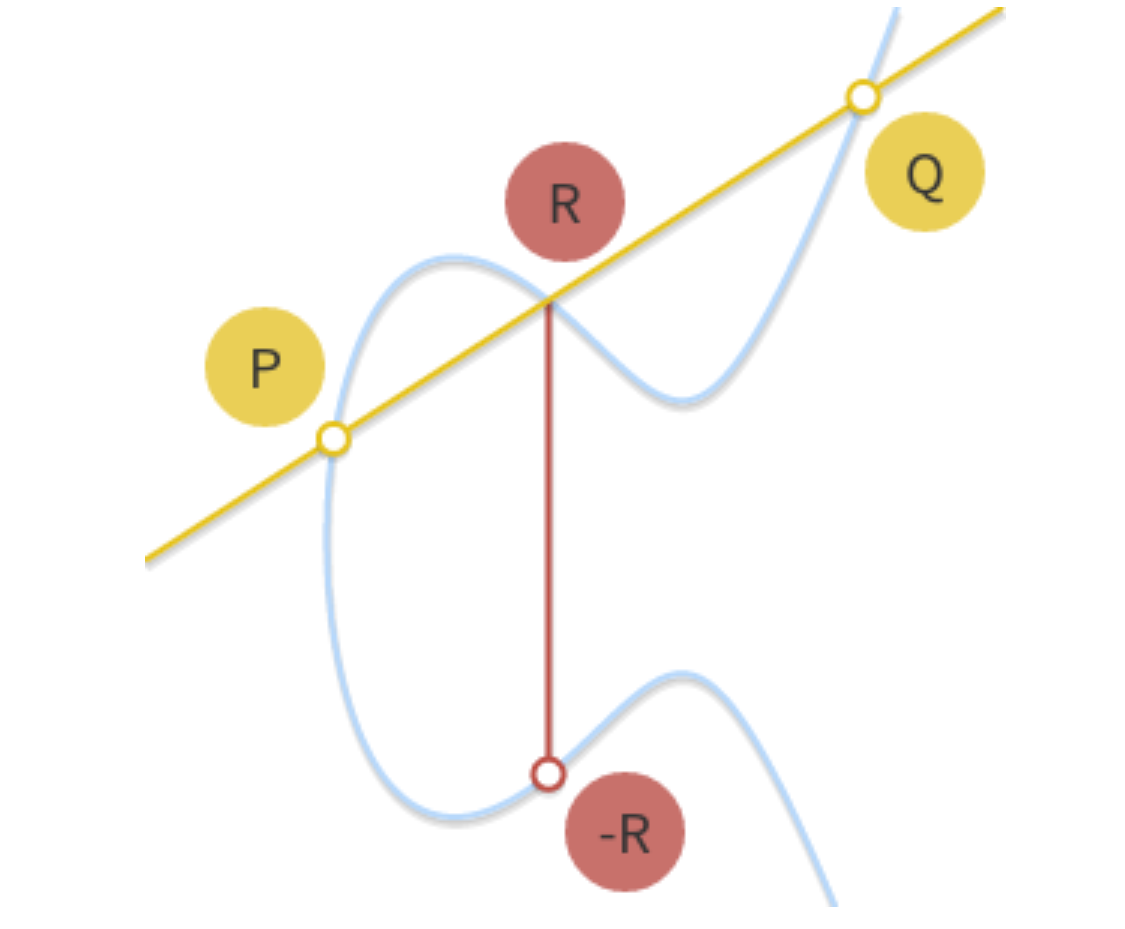
\includegraphics[scale=0.7]{add3.PNG}
    \item Here, P+Q=-R, and this is how ECC works (In case you would love to play with point adition and scalar multiplication using visual tool, here is one such thing - https://andrea.corbellini.name/ecc/interactive/reals-add.html 
    \item  And unsurprisingly, we can add one point to itself too \item How many steps would it take to compute x•P, where x is a random 256-bit integer? In this case, x can range anywhere from 0 to $1.1579209e+77$.
    It turns out that computing x•P would never require more than 510 point addition operations. Here’s why. First, compute the following series:
    $2^0•P, 2^1•P, 2^2•P, 2^3•P, 2^4•P, 2^{255}•P-1$
    \item We can define a group over elliptic curves where the elements of the group are the points of an elliptic curve;
    the identity element is the point at infinity 0;
    the inverse of a point $P$ is the one symmetric about the $x$-axis and addition is given by the following rule, that given three aligned non zero points $P,Q,R$, there sum is $P+Q+R=0$
    \item If we actually need to do something, we need to turn this geometric method into an algebraic method, but actually it can be really tedious because it requires solving cubic equations, but it is also not computationally difficult or anything
    \item If we are given $P$ and $n$, we have at least one polynomial time algorithm for computing $Q=nP$, but if we are given $Q$ and $P$ can we define $n$?This is known as logarithm problem. If we play with scalar multiplication for quite a while, we will even see some patterns from which we might think that we can come up with an algorithm which can solve this task. But there is a variant of this logarithm problem known as discrete logarithm problem, where we will see that if we reduce the domain of elliptic curves, the scalar multiplication still remains easy but discrete log become really a hard problem
\end{itemize}
\section{Elliptic Curves in $F_p$}
As a refresher, in fields we have two binary operations: addition (+) and multiplication (·). Both are closed, associative and commutative. For both operations, there exist a unique identity element, and for every element there's a unique inverse element. Finally, multiplication is distributive over the addition, $x.(y+z)=x.y+x.z$
From earlier intro, we actually defined elliptic curves as  $\begin{array}{rcl}
  \left\{(x, y) \in \mathbb{R}^2 \right. & \left. | \right. & \left. y^2 = x^3 + ax + b, \right. \\
  & & \left. 4a^3 + 27b^2 \ne 0\right\}\ \cup\ \left\{0\right\}
\end{array}$\\
Since we have restricted elliptic curves to finite fields, now we will say, \\
$\begin{array}{rcl}
  \left\{(x, y) \in (\mathbb{F}_p)^2 \right. & \left. | \right. & \left. y^2 \equiv x^3 + ax + b \pmod{p}, \right. \\
  & & \left. 4a^3 + 27b^2 \not\equiv 0 \pmod{p}\right\}\ \cup\ \left\{0\right\}
\end{array}$ where 0(or the identity element) is still the point at infinity, and $a$ and $b$  are two integers $F_p$, So what previously was a continuous curve is now a set of disjoint points in the $xy$-plane. Even if we have restricted our domain, elliptic curves in still form an abelian group. When it comes to point addition, clearly we need to change a bit our definition of addition in order to make it work in $F_p$. We can informally say that a line in $F_p$ is the set of points satisfying $ax+by+c=0(mod p)$.

The order of an elliptic curve group is the number of points in a group and we can find that using a fairly efficient algorithm (Schoof's algorithm)

\section{Scalar Multiplication and Cyclic Subgroups}
Multiplication over points for elliptic curves in $F_p$ has an interesting property. Take the curve $y^2 \equiv x^3 + 2x + 3 \pmod{97}$ and a point $P=(3,6)$. If we calculate the multiples of $p$, 
\begin{itemize}
    \item $0P=0$
    \item $1P=(3,6)$
    \item $2P=(80,10)$
    \item $3P=(80,87)$
    \item $4P=(3,91)$
    \item $5P=0$
    \item $6P=(3,6)$ and so on
\end{itemize}
    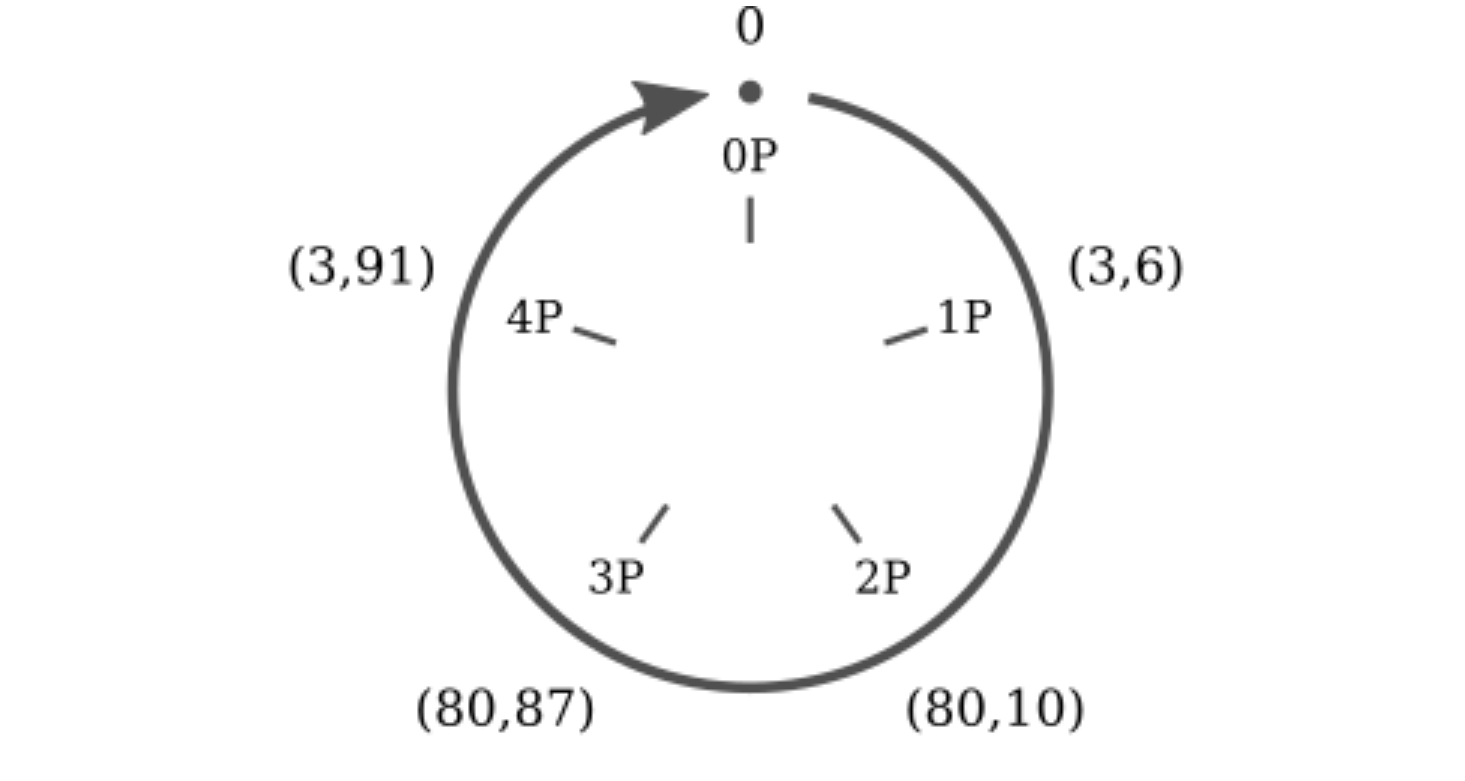
\includegraphics[scale=0.8]{add2.PNG}\\
We can immediately see two things: firstly, the multiples of  are just five: the other points of the elliptic curve never appear. Secondly, they are repeating cyclically and we can write $kP = (k \bmod{5})P$ and the point $P$ is called generator or base point of the cyclic subgroup.

Now the next thing immediately appearing in our mind is what is the order of the sub group generated by point $P$ and how we find that. Apparently, Schoof's algorithm can't be applied directly but we can take help from it sure :) In fact the order of a sub group generated by $P$ is the smallest $n$ such that $nP=0$, in above example which is $5$ and the order of $P$ is linked to the order of EC according to Lagrange's theorem, which states that the order of a subgroup is a divisor of the order of the parent group. In other words, if an elliptic curve contains $N$ points and one of its sub group contains $n$ points, then $n|N$. So these two information helps us find an obvious way to figure out such an $n$ yayy :D 
\section{But what is a good base point!?}
For our ECC algorithms, we want subgroups with a high order. So in general we will choose an elliptic curve, calculate its order $N$, choose a high divisor as the subgroup order $n$ and find a suitable base point. So we do not find a base point and then find its order, it's the other way around.

Oops but we need to define one more thing: co factor. Lagrange's theorem implies that the number $h=\frac{N}{n}$ is always an integer (because $n$ is a divisor of $N$). The number $h$ has a name: it's the co-factor of the subgroup.
Since for every point on the EC, we have $NP=0$, we can write $n(hP)=0$. Now say, $G=hP$, then if $n$ is prime, apparently, $G$ creates a sub group of order $n$(except when $G=hP=0$)
\section{Back to Discrete Logarithm}
We defined this problem earlier. Interestingly, it is *hard* that because is no known polynomial time algorithm for this problem. What makes ECC interesting is that, as of today, the discrete logarithm problem for elliptic curves seems to be "harder" if compared to other similar problems used in cryptography. This implies that we need fewer bits to achieve the same level of security as with other cryptosystems.

\section{Domain Parameters}
Our elliptic curve algorithms will work in a cyclic subgroup of an elliptic curve over a finite field. So we need $6$ different parameters, prime $p$ specifying the size of the field, co efficient $a$ and $b$, base point $G$, order $n$ of the sub group, co factor $h$ of the sub group.
\section{Are All Curves Good}
There are some classes of elliptic curves which are weak and allow the use of special purpose algorithms to solve the discrete logarithm problem efficiently. For example, all the curves that have $p=hn$ (when the order of the finite field is equal to the order of the elliptic curve) are vulnerable to Smart's attack, which can be used to solve discrete logarithms in polynomial time on a classical computer.

Now, if anyone gives you the domain parameters of a curve. there's the possibility that provider has discovered a new class of weak curves that nobody knows and built a "fast" algorithm for computing discrete logarithms on the curve provider gave you. How can the provider convinces you of the contrary, that it is not aware of any vulnerability?

To solve this kind of problem, sometimes we have an additional domain parameter: the seed $S$. This is a random number used to generate the coefficients $a$ and $b$, or the base point $G$, or both. These parameters are generated by computing the hash of the seed $S$. Hashes, as we know, are "easy" to compute, but "hard" to reverse.\\
$S= random()\\
 H = hash(S)\\
 a = f(H)\\
 b = g(H)$\\
 If we wanted to cheat and try to construct a seed from the domain parameters, we would have to solve a "hard" problem: hash inversion.
 
 \section{Elliptic Curve Cryptography}
Poof! We are finally here!
\begin{itemize}
    \item The private key is a random integer $d$ chosen from $\{1,2,\dots n-1\}$  (where $n$ is the order of the subgroup).
    \item The public key is the point $H=dG$ (where $G$ is the base point of the subgroup)
\end{itemize}
\section{Encryption with ECDH}
It is actually a key-agreement protocol, more than an encryption algorithm. This basically means that ECDH defines (to some extent) how keys should be generated and exchanged between parties. How we encrypt data using such keys is up to us.

The problem it solves is the following: two parties (the usual Alice and Bob) want to exchange information securely, so that a third party (M) may intercept them, but may not decode them. 

Here is how it works -
\begin{itemize}
    \item Alice and Bob generate their own private and public keys. We have the private key $d_A$ and the public key $H_A=d_AG$ for Alice, and the keys $d_B$  and $H_B=d_BG$ for Bob. Note that both Alice and Bob are using the same domain parameters: the same base point on the same elliptic curve on the same finite field.
    \item Alice and Bob exchange their public keys $H_A$  and $H_B$ over an insecure channel. M would intercept $H_A$ and $H_B$, but won't be able to find out neither $d_A$ nor $d_B$ without solving the discrete logarithm problem.
    \item Alice calculates $S=d_AH_B$ (using her own private key and Bob's public key), and Bob calculates $S=d_BH_A$ and clearly $S$ is the same for both
\end{itemize}
Now the question if M can infer anything about $S$ given $G$, $H_A$ and $H_B$. This is in fact The Diffie-Hellman problem for elliptic curves is assumed to be a "hard" problem. It is believed to be as "hard" as the discrete logarithm problem, although no mathematical proofs are available.
\section{Signing with ECDSA}
The scenario is the following: Alice wants to sign a message with her private key ($d_A$), and Bob wants to validate the signature using Alice's public key ($H_A$). Nobody but Alice should be able to produce valid signatures. Everyone should be able to check signatures.
ECDSA works on the hash of the message than on the message itself, but the hash needs to cryptographically secure. The hash of the message needs to be truncated so that the bit length of the hash is the same as the bit length of $n$ (the order of the subgroup). The truncated hash is an integer and will be denoted as $z$. 
The algorithm Alice uses for signing is the following- 
\begin{itemize}
    \item Take a random integer $k$ chosen from $\{1,2,\dots n-1\}$ (where $n$ is the subgroup order).
    \item calculate $P=kG$, $G$ being the base point of the subgroup
    \item Calculate $r = x_P \bmod{n}$, $x_P$ is the $x$ co ordinate of $P$, if $r=0$ then try again
    \item Calculate $s = k^{-1} (z + rd_A) \bmod{n}$, if $s=0$ then try again
\end{itemize}
\section{Verifying Signatures}
In order to verify the signature we'll need Alice's public key$H_A$, the (truncated) hash $z$ and, obviously, the signature $(r,s)$.
\begin{itemize}
    \item Calculate $u_1 = s^{-1} z \bmod{n}$
    \item Calculate $u_2 = s^{-1} r \bmod{n}$
    \item Calculate $P = u_1 G + u_2 H_A$
\end{itemize}
Now find $x_P$ and the sign is valid iff $r = x_P \bmod{n}$
\section{Correctness of the Algorithm}
In order to know whether this is correct, we just need to make sure that the point P in verifying signature part is the same as the signature generation algorithm.
We can write:\\
\begin{align*}
  P & = u_1 G + u_2 H_A \\
    & = u_1 G + u_2 d_A G \\
    & = (u_1 + u_2 d_A) G
\end{align*}
Using the definition from above, we can further write
\begin{align*}
  P & = (u_1 + u_2 d_A) G \\
    & = (s^{-1} z + s^{-1} r d_A) G \\
    & = s^{-1} (z + r d_A) G
\end{align*}
We know $s = k^{-1} (z + rd_A) \bmod{n}$. Modifying we can get $k = s^{-1} (z + rd_A) \bmod{n}$. Substituting the result in the equation, \begin{align*}
  P & = s^{-1} (z + r d_A) G \\
    & = k G
\end{align*}
Exactly what we have expected !
\section{What $k$ to choose}
We need to make sure that $k$s we are generating are really from a good *random* number generator and truly random.
If we use the same $k$ for all signatures, or if our random number generator were somewhat predictable, an attacker would be able to find out the private key and he would just need two signatures for that, say $(r_1,s_1)$ and $(r_2,s_2)$
together with the domain parameters, which will be the same and in fact $k$ is the same here. 
\begin{itemize}
    \item Note that $r_1 = r_2$ because $P_1=kG=P_2$ and $r = x_P \bmod{n}$ 
    \item $(s_1 - s_2) \bmod{n} = k^{-1} (z_1 - z_2) \bmod{n}$, this equation follows directly from the equation of $s$
    \item Rearranging, we get $k = (z_1 - z_2)(s_1 - s_2)^{-1} \bmod{n}$
\end{itemize}
Now we can find the value of the private key $d$ from the equations introduced before, $s = k^{-1}(z + rd) \bmod{n}\ \ \Rightarrow\ \ d = r^{-1} (sk - z) \bmod{n}$ 
\section{Let's Break Discrete Logarithm Problem}
As a fresher, given two points $P$ and $Q$,find out the integer $x$ that satisfies the equation $Q=xP$. The points belong to a subgroup of an elliptic curve, which has a base point $G$ and whose order is $n$.
\subsection{Baby Step Giant Step Algorithm}
We can write any integer $x$ such that $x=am+b$. So we can say:
\begin{align*}
  Q & = xP \\
  Q & = (am + b) P \\
  Q & = am P + b P \\
  Q - am P & = b P
\end{align*}
The algorithm is the following - 
\begin{itemize}
    \item Calculate $m = \left\lceil{\sqrt{n}}\right\rceil$
    \item For every b in $0,1,\dots m$ calculate $bP$ and store the result in a hash table
    \item For every a in $0,1,2\dots m$:
    \begin{itemize}
        \item Calculate $amP$
        \item Calculate $Q-amP$
        \item Check the hash table to see if there exists a point $bP$ such that $Q-amP=bP$
    \end{itemize}
\end{itemize}
If we look at what this algorithm is doing, we will see that when $a=0$, we have been checking whether $Q$ is among $0P$ to $mP$, when $a=1$, we are checking whether $Q$ is among $mP$ to $2mP$ and so on and this way finally from $(m-1)P$ to $m^2P$ or roughly $nP$.

Since look up takes constant time, the algorithm has both time and space complexity $O(\sqrt{n})$ or $O(2^{k/2})$, if you consider that $n$ has $k$ bits. Now let's try to see how huge this number is :')

Let's take a standardized curve: prime192v1 (aka secp192r1, ansiX9p192r1). This curve has order $n=0xffffffffffffffff ffffffff99def836146bc9b1\\b4d22831$.Suppose each point needs exactly 32 bytes: our hash table would need approximately $2.5*10^{30}$ bytes of memory. Looking on the web, it seems that the total world storage capacity is in the order of the zettabyte ($10^{21}$ bytes). Imagine trying to store this thing poof :(
\subsection{Pollard's $\rho$}
Here we attempt to solve a slightly different problem, when we are asked to find $x$ given that $Q=xP$, we try to solve given $Q,P$ can we find $a,b,A,B$ such that $aP+bQ=AP+BQ$
If we find such four things, we can write- 
\begin{align*}
  aP + bQ & = AP + BQ \\
  aP + bxP & = AP + BxP \\
  (a + bx) P & = (A + Bx) P \\
  (a - A) P & = (B - b) xP
\end{align*}
We can get rid of $P$. Recall that our subgroup is cyclic with order $n$, so we can write -
\begin{align*}
  a - A & \equiv (B - b) x \pmod{n} \\
  x & = (a - A)(B - b)^{-1} \bmod{n}
\end{align*}
Now how to find $a,b,A,B$? The principle of operation of Pollard's rho is simple: we generate a pseudo-random sequence of points $X_1,X_2,\dots$ where each $X_i=a_iP+b_iQ$ The sequence can be generated using a pseudo-random function $f$ like this:\\
$(a_{i + 1}, b_{i + 1}) = f(X_i)$\\
It doesn't really matter how $f$ works internally (although certain functions may yield results faster than others), what matters is that $f$ determines the next point in the sequence based on the previous one, and that all the $a_i$ and $b_i$ coefficients are known by us.
By using such $f$, sooner or later we will see a loop in our sequence. That is, we will see a point $X_j=X_i$.The reason why we must see the cycle is simple: the number of points is finite, hence they must repeat sooner or later. Once we see where the cycle is, we can use the equations above to figure out the discrete logarithm. Now how to detect cycle efficiently?
\subsubsection{Tortoise and Hare Algorithm}
The main idea is that We take two pets, the tortoise and the hare, and make them walk our sequence of points from left to right. The tortoise is slow and reads each point one by one; the hare is fast and skips a point at every step. After some time both the tortoise and the hare will have found the same point, but with different coefficient pairs. Or, to express that with equations, the tortoise will have found a pair $(a,b)$ and the hare will have found a pair $(A,B)$ such that $aP + bQ = AP + BQ$.

It's easy to see that this algorithm requires constant memory. Calculating the asymptotic time complexity is not that easy, but a probabilistic proof that shows how the time complexity is $O(\sqrt{n})$ as we have already said. The proof is based on the "birthday paradox", which is about the probability of two people having the same birthday.

Now since this is good on the aspect of space, let's consider how much it would take to break it. As we have already said, prime192v1 is one of the "smallest" elliptic curves(Has the smallest order among standardized curves). We also said that Pollard's $\rho$ has  time complexity $O(\sqrt{n})$. If we used the same technique as Chris Monico(who used the parallelized version of pollard's $rho$ to break $109$ bit long curve and that took $17$ months calendar time) (the same algorithm, on the same hardware, with the same number of machines), how much would it take to compute a logarithm on prime192v1?
$17\ \text{months}\ \times \frac{\sqrt{2^{192}}}{\sqrt{2^{109}}} \approx 5 \cdot 10^{13}\ \text{months}$
\section{Tomorrow's Techniques}
\subsection{Shor's Algorithm}
Tomorrow's techniques are a bit more worrisome: there exists a quantum algorithm capable of computing discrete logarithms in polynomial time: Shor's algorithm, which has time complexity $O((\log n)^3)$ and space complexity $O(\log n)$

Quantum computers are still not sophisticated enough to run algorithms like Shor's, still the need for quantum-resistant algorithms may be something worth investigating now. What we encrypt today might not be safe tomorrow.
\section{Why ECC}
Long story short, in order to achieve the same level of security ECC requires way less number of bits than RSA and smol things are easy to maintain :')
\section{Acknowledgement}
I combined ideas and information from multiple articles online and tried to put what I found most useful and enjoyable :)
\end{document}
